\subsection{Non-Overlapping Subdomains}

\subsubsection{Introduction}

When dealing with \definition{Non Overlapping Subdomains}, the computational \textbf{domain is divided into adjacent subdomains that share a common\break boundary, but do \underline{not overlap}}. This approach simplifies the handling of subdomain interfaces and ensures a clear distinction between different regions of the domain.

\highspace
\begin{flushleft}
    \textcolor{Green3}{\faIcon{tools} \textbf{Key Characteristics of Non-Overlapping Subdomains}}
\end{flushleft}
\begin{enumerate}
    \item \textbf{Adjacent Subdomains}. The domain is divided into subdomains $\Omega_{1}$ and $\Omega_{2}$ that are \emph{adjacent} to each other. These subdomains touch each other \emph{only} along their common boundary $\Gamma$, but do \emph{not overlap}.
    \begin{figure}[!htp]
        \centering
        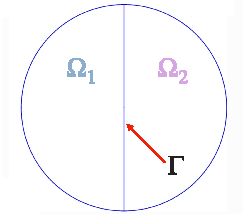
\includegraphics[width=.3\textwidth]{img/non-overlapping-subdomains-1.pdf}
    \end{figure}
    
    \item \textbf{Partitioning Indices}. Each subdomain has its own set of interior nodes. The indices of these nodes are divided as follows:
    \begin{itemize}
        \item $S_{1}$: Indices of interior nodes in $\Omega_{1}$.
        \item $S_{2}$: Indices of interior nodes in $\Omega_{2}$.
    \end{itemize}
    The nodes that lie on the boundary $\Gamma$ between the two subdomains are indexed by:
    \begin{itemize}
        \item $S_{\Gamma}$: Indices corresponding to the interface nodes along $\Gamma$.
    \end{itemize}
    \begin{figure}[!htp]
        \centering
        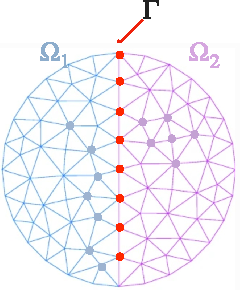
\includegraphics[width=.3\textwidth]{img/non-overlapping-subdomains-2.pdf}
    \end{figure}

    \newpage

    \item \textbf{Zero Blocks}. Nodes in $\Omega_{1}$ are not directly connected to nodes in $\Omega_{2}$; they are connected only through the interface nodes in $\Gamma$. This results in zero blocks in the off-diagonal positions of the matrix for direct connections between $\Omega_{1}$ and $\Omega_{2}$.
    
    \item \textbf{Symmetric Block Linear System}. The matrix $A$ and the solution vector $x$ are partitioned into blocks corresponding to $\Omega_{1}$, $\Omega_{2}$ and $\Gamma$:
    \begin{equation*}
        \begin{bmatrix}
            A_{11} & 0 & A_{1\Gamma} \\
            0 & A_{22} & A_{2\Gamma} \\
            A_{1\Gamma}^{T} & A_{2\Gamma}^{T} & A_{\Gamma\Gamma}
        \end{bmatrix}
        \begin{bmatrix}
            \mathbf{x}_{1} \\ \mathbf{x}_{2} \\ \mathbf{x}_{\Gamma}
        \end{bmatrix}
        =
        \begin{bmatrix}
            \mathbf{b}_{1} \\ \mathbf{b}_{2} \\ \mathbf{b}_{\Gamma}
        \end{bmatrix}
    \end{equation*}
    \begin{itemize}
        \item $A_{11}$: Matrix block corresponding to the interior nodes in $\Omega_{1}$.
        \item $A_{22}$: Matrix block corresponding to the interior nodes in $\Omega_{2}$.
        \item $A_{1\Gamma}$ and $A_{2\Gamma}$: Matrix blocks corresponding to the connections between the interior nodes of $\Omega_{1}$ and $\Omega_{2}$ with the interface nodes in $\Gamma$.
        \item $A_{\Gamma\Gamma}$: Matrix block corresponding to the interface nodes in $\Gamma$.
    \end{itemize}
    The right-hand-side vector $\mathbf{b}$ is similarly partitioned into $\mathbf{b}_{1}$, $\mathbf{b}_{2}$, and $\mathbf{b}_\Gamma$, corresponding to the components in each subdomain and the interface.

    \item \textbf{Algorithmic Approach}. When using non-overlapping subdomains, the \textbf{main goal is to solve the PDE in each subdomain independently while ensuring the interface conditions are satisfied}. Iterative solvers can be employed to update the solution at each step, ensuring that boundary conditions between subdomains are consistently respected.
\end{enumerate}
